\documentclass[aspectratio=169]{beamer}

\usetheme{Madrid}
\usecolortheme{seahorse}
\usepackage{amsmath, amssymb}
\usepackage{tikz}
\usepackage{pgfplots}
\pgfplotsset{compat=1.18}
\usepackage{xcolor}
\usepackage{booktabs}
\usepackage{array}

% Custom colours matching a clean academic look
\definecolor{statblue}{RGB}{31, 73, 125}
\definecolor{statorange}{RGB}{210, 105, 30}
\definecolor{statgreen}{RGB}{34, 120, 60}

\setbeamercolor{frametitle}{bg=statblue, fg=white}
\setbeamercolor{title}{bg=statblue, fg=white}
\setbeamercolor{block title}{bg=statblue!80, fg=white}
\setbeamercolor{block title alerted}{bg=statorange!90, fg=white}
\setbeamercolor{block title example}{bg=statgreen!80, fg=white}
\setbeamercolor{item}{fg=statblue}
\setbeamercolor{subitem}{fg=statorange}

\title{The Central Limit Theorem}
\subtitle{Statistics 12 --- A 90-Minute Lesson}
\author{}
\date{}

\begin{document}

% -------------------------------------------------------
\begin{frame}
    \titlepage
\end{frame}

% -------------------------------------------------------
\begin{frame}{Lesson Goals}
    By the end of this lesson, students should be able to:
    \begin{itemize}
        \item explain what a \textbf{sampling distribution} is
        \item state the Central Limit Theorem (CLT) precisely
        \item identify the \textbf{mean} and \textbf{standard error} of a sampling distribution
        \item recognise when the CLT applies
        \item use the CLT to calculate probabilities about sample means
        \item distinguish between the distribution of \emph{individuals} and the
              distribution of \emph{sample means}
    \end{itemize}
\end{frame}

% -------------------------------------------------------
\begin{frame}{Suggested Timing}
    \begin{center}
        \begin{tabular}{@{}ll@{}}
            \toprule
            \textbf{Time} & \textbf{Activity}                                \\
            \midrule
            0--5 min      & Hook: the dice simulation                        \\
            5--20 min     & Sampling distributions --- concept \& vocabulary \\
            20--35 min    & The CLT statement \& parameters                  \\
            35--50 min    & Worked examples                                  \\
            50--60 min    & Think-pair-share \& misconceptions               \\
            60--75 min    & More worked examples (harder)                    \\
            75--85 min    & Student practice                                 \\
            85--90 min    & Summary \& exit card                             \\
            \bottomrule
        \end{tabular}
    \end{center}
\end{frame}

% -------------------------------------------------------
\section{Motivation}

\begin{frame}{Hook: Rolling Dice}
    \begin{columns}
        \column{0.55\textwidth}
        Imagine rolling \textbf{one fair die} many times.
        \begin{itemize}
            \item Each outcome (1--6) is equally likely.
            \item The distribution is \textbf{uniform} --- definitely not bell-shaped.
        \end{itemize}
        \bigskip
        Now imagine rolling \textbf{30 dice} and recording the \emph{average}.
        \begin{itemize}
            \item Repeat this experiment thousands of times.
            \item What shape do you expect for the distribution of averages?
        \end{itemize}
        \column{0.42\textwidth}
        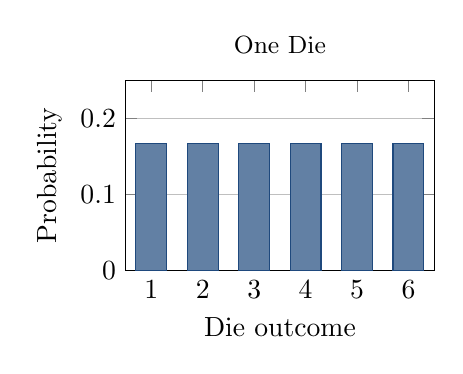
\begin{tikzpicture}
            \begin{axis}[
                    width=5.5cm, height=4cm,
                    xlabel={Die outcome}, ylabel={Probability},
                    ymin=0, ymax=0.25,
                    xtick={1,2,3,4,5,6},
                    bar width=0.6,
                    ymajorgrids=true,
                    title={\small One Die},
                    title style={font=\small}
                ]
                \addplot[ybar, fill=statblue!70, draw=statblue] coordinates
                    {(1,0.167)(2,0.167)(3,0.167)(4,0.167)(5,0.167)(6,0.167)};
            \end{axis}
        \end{tikzpicture}
    \end{columns}
    \medskip
    \begin{alertblock}{The surprising answer}
        The distribution of sample averages will look approximately \textbf{normal},
        no matter the shape of the original population!
    \end{alertblock}
\end{frame}

% -------------------------------------------------------
\section{Sampling Distributions}

\begin{frame}{Key Vocabulary}
    \begin{block}{Population}
        The complete set of individuals or measurements we are interested in.
    \end{block}
    \begin{block}{Sample}
        A subset of the population that we actually observe.
    \end{block}
    \begin{block}{Statistic}
        A number computed from a sample (e.g.\ the sample mean $\bar{x}$).
    \end{block}
    \begin{alertblock}{Sampling Distribution}
        The distribution of a statistic over \emph{all possible samples of the same size}
        drawn from the same population.
    \end{alertblock}
    \medskip
    \small Key insight: because samples vary, statistics vary. A sampling distribution
    describes \emph{how much} and \emph{in what pattern}.
\end{frame}

% -------------------------------------------------------
\begin{frame}{Population vs.\ Sampling Distribution}
    \begin{columns}
        \column{0.48\textwidth}
        \begin{exampleblock}{Distribution of individuals}
            \begin{itemize}
                \item Describes one observation chosen at random
                \item Mean: $\mu$
                \item Standard deviation: $\sigma$
                \item Can be any shape
            \end{itemize}
        \end{exampleblock}
        \column{0.48\textwidth}
        \begin{alertblock}{Sampling distribution of $\bar{x}$}
            \begin{itemize}
                \item Describes the mean of a sample of size $n$
                \item Mean: $\mu_{\bar{x}} = \mu$
                \item Standard deviation: $\sigma_{\bar{x}} = \dfrac{\sigma}{\sqrt{n}}$
                \item Approximately normal (CLT!)
            \end{itemize}
        \end{alertblock}
    \end{columns}
    \bigskip
    \begin{block}{Standard Error}
        The quantity $\dfrac{\sigma}{\sqrt{n}}$ is called the \textbf{standard error} (SE) of the mean.
        It measures how much $\bar{x}$ typically varies from sample to sample.
    \end{block}
\end{frame}

% -------------------------------------------------------
\section{The Central Limit Theorem}

\begin{frame}{The Central Limit Theorem --- Statement}
    \begin{alertblock}{Central Limit Theorem (CLT)}
        Let $X_1, X_2, \ldots, X_n$ be a random sample from \emph{any} population with
        mean $\mu$ and finite standard deviation $\sigma$.  When $n$ is sufficiently large,
        the sampling distribution of the sample mean $\bar{X}$ is approximately normal:
        \[
            \bar{X} \;\approx\; N\!\left(\mu,\; \frac{\sigma}{\sqrt{n}}\right)
        \]
        The approximation improves as $n$ increases.
    \end{alertblock}
    \medskip
    Three things the CLT tells us about $\bar{X}$:
    \begin{enumerate}
        \item \textbf{Shape:} approximately normal
        \item \textbf{Centre:} mean equals the population mean $\mu$
        \item \textbf{Spread:} standard deviation equals $\dfrac{\sigma}{\sqrt{n}}$
    \end{enumerate}
\end{frame}

% -------------------------------------------------------
\begin{frame}{When Does the CLT Apply?}
    \begin{columns}
        \column{0.55\textwidth}
        \begin{block}{The usual guideline}
            $n \geq 30$ is sufficient for most populations.
        \end{block}
        \medskip
        \begin{itemize}
            \item If the population is already \textbf{normal}, the CLT holds for \emph{any} $n$.
            \item For \textbf{mildly skewed} populations, $n \approx 15$--$20$ may suffice.
            \item For \textbf{heavily skewed} or unusual populations, you may need $n > 30$.
        \end{itemize}
        \column{0.42\textwidth}
        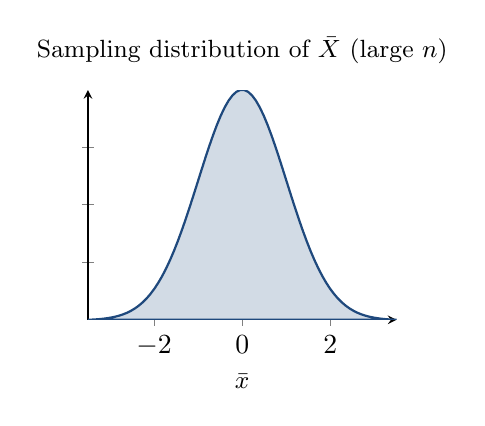
\begin{tikzpicture}
            \begin{axis}[
                    width=5.5cm, height=4.5cm,
                    domain=-3.5:3.5,
                    samples=80,
                    xlabel={$\bar{x}$}, ylabel={},
                    yticklabels={},
                    axis lines=left,
                    title={\small Sampling distribution of $\bar{X}$ (large $n$)},
                    title style={font=\scriptsize},
                    xlabel style={font=\small}
                ]
                \addplot[thick, statblue, fill=statblue!20] {exp(-x^2/2)/sqrt(2*pi)} \closedcycle;
            \end{axis}
        \end{tikzpicture}
    \end{columns}
    \medskip
    \begin{alertblock}{Important caveat}
        The CLT applies to the distribution of \emph{sample means}, not to individual values.
    \end{alertblock}
\end{frame}

% -------------------------------------------------------
\begin{frame}{Why the Standard Error Shrinks}
    The standard error $\dfrac{\sigma}{\sqrt{n}}$ decreases as $n$ grows.
    \medskip

    \begin{center}
        \begin{tabular}{@{}cccc@{}}
            \toprule
            $n$ & $\sigma = 10$ & SE $= \sigma/\sqrt{n}$ & Relative to $n=1$ \\
            \midrule
            1   & 10            & 10.00                  & 100\%             \\
            4   & 10            & 5.00                   & 50\%              \\
            25  & 10            & 2.00                   & 20\%              \\
            100 & 10            & 1.00                   & 10\%              \\
            400 & 10            & 0.50                   & 5\%               \\
            \bottomrule
        \end{tabular}
    \end{center}
    \medskip
    \begin{itemize}
        \item To \textbf{halve} the standard error, you must \textbf{quadruple} the sample size.
        \item Larger samples give more precise estimates of $\mu$.
    \end{itemize}
\end{frame}

% -------------------------------------------------------
\section{Worked Examples}

\begin{frame}{Using the CLT --- The Z-Score for $\bar{X}$}
    \begin{block}{Standardising a sample mean}
        To find probabilities about $\bar{X}$, convert to a $z$-score using:
        \[
            z = \frac{\bar{x} - \mu}{\sigma / \sqrt{n}}
        \]
        Then use a standard normal table or calculator.
    \end{block}
    \medskip
    \textbf{Compare:}
    \begin{itemize}
        \item For an individual: $z = \dfrac{x - \mu}{\sigma}$
        \item For a sample mean: $z = \dfrac{\bar{x} - \mu}{\sigma / \sqrt{n}}$
    \end{itemize}
    \medskip
    The only difference is the \textbf{denominator} --- we divide by the standard error,
    not $\sigma$.
\end{frame}

% -------------------------------------------------------
\begin{frame}{Worked Example 1: Coffee Shop Wait Times}
    \begin{exampleblock}{Problem}
        Wait times at a coffee shop are right-skewed with mean $\mu = 4.2$ min and
        standard deviation $\sigma = 1.8$ min.  A random sample of $n = 36$ customers
        is selected.  What is the probability that the sample mean wait time exceeds
        4.8 minutes?
    \end{exampleblock}

    \textbf{Step 1: Check CLT conditions.}
    $n = 36 \geq 30$. \checkmark

    \textbf{Step 2: Identify the sampling distribution.}
    \[
        \bar{X} \approx N\!\left(4.2,\; \frac{1.8}{\sqrt{36}}\right) = N(4.2,\; 0.3)
    \]

    \textbf{Step 3: Standardise.}
    \[
        z = \frac{4.8 - 4.2}{0.3} = \frac{0.6}{0.3} = 2.00
    \]

    \textbf{Step 4: Find the probability.}
    \[
        P(\bar{X} > 4.8) = P(Z > 2.00) = 1 - 0.9772 = \mathbf{0.0228}
    \]
\end{frame}

% -------------------------------------------------------
\begin{frame}{Worked Example 1: What Does This Mean?}
    \begin{columns}
        \column{0.52\textwidth}
        \begin{itemize}
            \item There is about a \textbf{2.3\% chance} that a sample of 36 customers has
                  a mean wait time above 4.8 minutes.
            \item This is quite unlikely --- a sample mean that far above $\mu$ would be
                  unusual.
            \item Notice: for an \emph{individual}, $P(X > 4.8)$ would be much larger.
        \end{itemize}
        \medskip
        \begin{alertblock}{Key point}
            Sample means are less variable than individual values.
        \end{alertblock}
        \column{0.45\textwidth}
        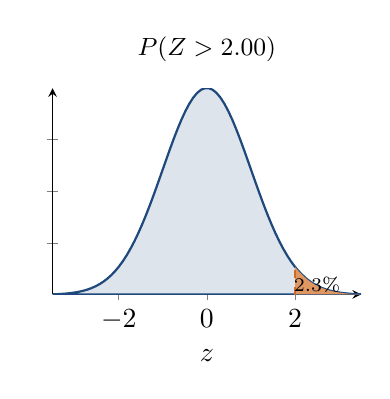
\begin{tikzpicture}
            \begin{axis}[
                    width=5.5cm, height=4.2cm,
                    domain=-3.5:3.5, samples=80,
                    xlabel={$z$}, ylabel={},
                    yticklabels={}, axis lines=left,
                    title={\small $P(Z>2.00)$},
                    title style={font=\small}
                ]
                \addplot[thick, statblue, fill=statblue!15, domain=-3.5:3.5]
                {exp(-x^2/2)/sqrt(2*pi)} \closedcycle;
                \addplot[fill=statorange!70, draw=none, domain=2:3.5]
                {exp(-x^2/2)/sqrt(2*pi)} \closedcycle;
                \draw[dashed, thick, statorange] (axis cs:2,0) -- (axis cs:2,0.054);
                \node[font=\scriptsize] at (axis cs:2.5, 0.02) {2.3\%};
            \end{axis}
        \end{tikzpicture}
    \end{columns}
\end{frame}

% -------------------------------------------------------
\begin{frame}{Worked Example 2: Heights of Students}
    \begin{exampleblock}{Problem}
        Heights of male students are normally distributed with $\mu = 175$ cm and
        $\sigma = 8$ cm.  A random sample of $n = 16$ male students is selected.

        \smallskip
        (a) Find $P(\bar{X} < 172)$.\\
        (b) Find $P(170 < \bar{X} < 178)$.
    \end{exampleblock}

    \textbf{Since the population is normal, CLT holds for any $n$.}

    \[
        \bar{X} \sim N\!\left(175,\; \frac{8}{\sqrt{16}}\right) = N(175,\; 2)
    \]

    \textbf{Part (a):}
    \[
        z = \frac{172 - 175}{2} = -1.5 \qquad
        P(\bar{X} < 172) = P(Z < -1.5) = \mathbf{0.0668}
    \]

    \textbf{Part (b):}
    \[
        z_1 = \frac{170-175}{2} = -2.5 \qquad z_2 = \frac{178-175}{2} = 1.5
    \]
    \[
        P(-2.5 < Z < 1.5) = 0.9332 - 0.0062 = \mathbf{0.9270}
    \]
\end{frame}

% -------------------------------------------------------
\begin{frame}{Think-Pair-Share: Spot the Mistake}
    \begin{alertblock}{A student wrote the following. What is wrong?}
        \textit{``The population of exam scores has mean 70 and standard deviation 15.
            A sample of $n = 25$ students is taken.
            The probability that a student scores above 75 is $P(Z > 1.33) \approx 0.092$.
            Therefore, about 9\% of sample means will be above 75.''}
    \end{alertblock}
    \bigskip
    \textbf{Discuss with a partner, then share your answer.}
    \bigskip
    \begin{block}{Hint}
        The student computed $z = \dfrac{75 - 70}{15} = 1.33$.
        Is this the right formula for a sample mean?
    \end{block}
\end{frame}

% -------------------------------------------------------
\begin{frame}{Think-Pair-Share: Correction}
    \begin{block}{What went wrong}
        The student used $z = \dfrac{\bar{x} - \mu}{\sigma}$ instead of
        $z = \dfrac{\bar{x} - \mu}{\sigma / \sqrt{n}}$.
    \end{block}

    \textbf{The correct calculation:}
    \[
        \text{SE} = \frac{15}{\sqrt{25}} = 3 \qquad
        z = \frac{75 - 70}{3} = 1.67
    \]
    \[
        P(\bar{X} > 75) = P(Z > 1.67) \approx 0.0475
    \]
    \medskip
    The probability is about \textbf{4.8\%}, not 9.2\%.

    \begin{alertblock}{Common error to avoid}
        When working with sample means, \emph{always} divide by
        $\dfrac{\sigma}{\sqrt{n}}$, not by $\sigma$ alone.
    \end{alertblock}
\end{frame}

% -------------------------------------------------------
\section{Harder Examples}

\begin{frame}{Worked Example 3: Finding a Boundary Value}
    \begin{exampleblock}{Problem}
        Monthly electricity bills in a city have mean \$120 and standard deviation \$25.
        A random sample of $n = 100$ bills is selected.
        Find the value $c$ such that $P(\bar{X} > c) = 0.05$.
    \end{exampleblock}

    \textbf{Step 1: Sampling distribution.}
    \[
        \bar{X} \approx N\!\left(120,\; \frac{25}{\sqrt{100}}\right) = N(120,\; 2.5)
    \]

    \textbf{Step 2: Find the $z$ value.} We need $P(Z > z^*) = 0.05$, so $z^* = 1.645$.

    \textbf{Step 3: Unstandardise.}
    \[
        c = \mu + z^* \cdot \frac{\sigma}{\sqrt{n}} = 120 + 1.645 \times 2.5 = 120 + 4.11 = \mathbf{\$124.11}
    \]

    \medskip
    Only 5\% of samples of size 100 would have a mean bill above \$124.11.
\end{frame}

% -------------------------------------------------------
\begin{frame}{Worked Example 4: Two Populations}
    \begin{exampleblock}{Problem}
        Brand A batteries have mean life $\mu_A = 500$ h, $\sigma_A = 40$ h.\\
        Brand B batteries have mean life $\mu_B = 490$ h, $\sigma_B = 30$ h.\\
        Samples of $n = 64$ batteries from each brand are tested independently.
        What is the probability that Brand A's sample mean exceeds Brand B's by more
        than 20 hours?
    \end{exampleblock}

    Let $D = \bar{X}_A - \bar{X}_B$.  By the CLT:
    \[
        E[D] = 500 - 490 = 10 \qquad
        \text{SD}(D) = \sqrt{\frac{40^2}{64} + \frac{30^2}{64}}
        = \sqrt{25 + 14.06} = \sqrt{39.06} \approx 6.25
    \]
    \[
        z = \frac{20 - 10}{6.25} = 1.60 \qquad
        P(D > 20) = P(Z > 1.60) \approx \mathbf{0.0548}
    \]
\end{frame}

% -------------------------------------------------------
\section{Practice}

\begin{frame}{Student Practice}
    Work on these problems individually or with a partner.
    \begin{enumerate}
        \item The weights of apples at a farm are distributed with $\mu = 182$ g and
              $\sigma = 14$ g.  A crate contains $n = 49$ apples chosen at random.
              \begin{enumerate}[(a)]
                  \item Find the mean and standard error of $\bar{X}$.
                  \item Find $P(\bar{X} > 185)$.
                  \item Find $P(179 < \bar{X} < 186)$.
              \end{enumerate}
        \item A random sample of $n = 64$ light bulbs is drawn from a population with
              $\mu = 800$ h and $\sigma = 80$ h.  Find the value $c$ such that
              $P(\bar{X} < c) = 0.90$.
        \item A population is strongly right-skewed with $\mu = 50$ and $\sigma = 10$.
              Can you apply the CLT to a sample of $n = 10$?  Explain your reasoning.
    \end{enumerate}
\end{frame}

% -------------------------------------------------------
\begin{frame}{Practice Solutions}
    \textbf{1.}
    (a) $\mu_{\bar{X}} = 182$ g, $\text{SE} = 14/\sqrt{49} = 2$ g.\medskip

    (b) $z = (185-182)/2 = 1.5 \Rightarrow P(\bar{X}>185) = P(Z>1.5) = 0.0668$.\medskip

    (c) $z_1 = (179-182)/2 = -1.5$, $z_2 = (186-182)/2 = 2.0$\\
    $P(-1.5 < Z < 2.0) = 0.9772 - 0.0668 = 0.9104$.
    \bigskip

    \textbf{2.} SE $= 80/\sqrt{64} = 10$.  Need $P(Z < z^*) = 0.90 \Rightarrow z^* = 1.282$.\\
    $c = 800 + 1.282 \times 10 = \mathbf{812.8}$ h.
    \bigskip

    \textbf{3.} No.  The guideline requires $n \geq 30$ for non-normal populations,
    and strongly skewed populations may need $n > 30$.  With $n = 10$, the CLT
    cannot reliably be applied here.
\end{frame}

% -------------------------------------------------------
\begin{frame}{Common Misconceptions}
    \begin{tabular}{@{}>{\bfseries}p{0.44\textwidth} p{0.5\textwidth}@{}}
        \toprule
        Misconception                                                      & Correction     \\
        \midrule
        ``The CLT says the population becomes normal.''                    &
        The CLT is about the \emph{sampling distribution of $\bar{X}$}, not the population. \\[6pt]
        ``A larger $n$ makes individual values less variable.''            &
        $n$ only reduces the variability of \emph{sample means}, not individuals.           \\[6pt]
        ``CLT requires the population to be symmetric.''                   &
        The CLT works for any shape, as long as $n$ is large enough.                        \\[6pt]
        ``$\sigma/\sqrt{n}$ is the standard deviation of the population.'' &
        It is the \emph{standard error} of $\bar{X}$, not $\sigma$.                         \\
        \bottomrule
    \end{tabular}
\end{frame}

% -------------------------------------------------------
\begin{frame}{Lesson Summary}
    \begin{block}{The Central Limit Theorem}
        For a random sample of size $n$ from a population with mean $\mu$ and
        standard deviation $\sigma$:
        \[
            \bar{X} \approx N\!\left(\mu,\; \frac{\sigma}{\sqrt{n}}\right)
            \quad \text{when } n \geq 30 \text{ (or population is normal)}
        \]
    \end{block}
    \medskip
    Key take-aways:
    \begin{itemize}
        \item The \textbf{mean} of $\bar{X}$ equals the population mean $\mu$.
        \item The \textbf{standard error} is $\sigma/\sqrt{n}$ --- it shrinks with larger $n$.
        \item Use $z = \dfrac{\bar{x} - \mu}{\sigma/\sqrt{n}}$ to find probabilities.
        \item The CLT applies regardless of population shape (for large $n$).
        \item The CLT is the foundation for \textbf{confidence intervals} and
              \textbf{hypothesis tests} (coming soon!).
    \end{itemize}
\end{frame}

% -------------------------------------------------------
\begin{frame}{Exit Card}
    Answer on a piece of paper before you leave.
    \begin{alertblock}{Question}
        The time (in minutes) students spend on homework each night has mean
        $\mu = 45$ min and standard deviation $\sigma = 12$ min.  A random sample of
        $n = 36$ students is selected.
        \begin{enumerate}[(a)]
            \item State the sampling distribution of $\bar{X}$, including its shape, mean,
                  and standard deviation.
            \item Find $P(\bar{X} > 48)$.
        \end{enumerate}
    \end{alertblock}
    \bigskip
    \begin{block}{Answer}
        (a) $\bar{X} \approx N(45,\; 2)$ since $12/\sqrt{36} = 2$.\quad
        (b) $z = (48-45)/2 = 1.5$;\quad $P(Z > 1.5) = 0.0668$.
    \end{block}
\end{frame}

\end{document}